\section{Generating Position, Mass and Velocity for Cluster Particles}
\label{Method:GeneratingPosMassVel}
\fxnote{write small intro}
\fxnote{in this section, we can introduce a generation of velocity, if we need that at some point}
\subsection{Gaussian Distributed Mass}
\fxnote{write here, what kind of distribution, we want!}

\begin{lstlisting}
void gaussian_mass_generator(vec (&mass), int number_of_particles)
{
  srand(time(NULL));
  for (int i = 0; i < number_of_particles; i++)
  {
  static int iset = 0;
  static double gset;
  double fac, rsq, v1, v2;
    do{
      v1 = 2.*((double) rand() / (RAND_MAX)) -1.0;
      v2 = 2.*((double) rand() / (RAND_MAX)) -1.0;
      rsq = v1*v1+v2*v2;
    } while (rsq >= 1.0 || rsq == 0.);
    fac = sqrt(-2.*log(rsq)/rsq);
    gset = v1*fac;
    iset = 1;
    mass(i) = v2*fac;
    mass(i) += 10;
  }
}
\end{lstlisting}

\begin{figure}[H]
\centering
	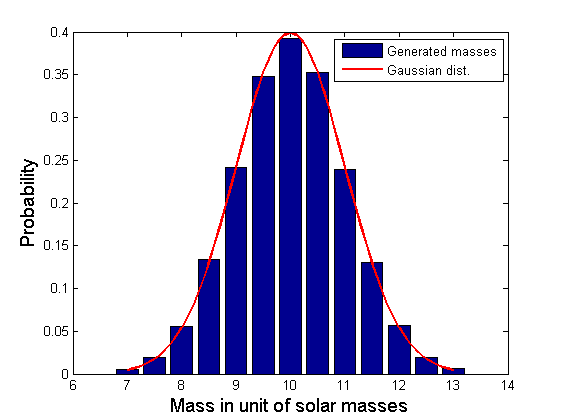
\includegraphics[width=0.7\linewidth]{Figures/random_mass_test.png}
\caption{
Histogram of the mass of 100,000 particles generated by the c++ code introduced \fxnote{where}. 
}
\label{fig:GaussianGeneratedMass}
\end{figure}
\fxnote{eq. include gaussian dist. in fig}

\subsection{Uniformly Distributed Position}
\fxnote{write here, what kind of distribution, we want!}

\begin{lstlisting}
void uniform_pos_generator(mat (&position), int N)
{
double pi=3.14159, c = 2*pi, R = 20;
vec phi(N), r(N), theta(N), x(N), y(N), v(N);

srand(time(NULL));

for (int i=0;i<N;i++){

        x(i) = ((double) rand() / (RAND_MAX)); //random numbers generated in the interval(0,1)
        y(i) = ((double) rand() / (RAND_MAX));
        v(i) = ((double) rand() / (RAND_MAX));
   }
for (int i=0;i<N;i++){
        phi(i)=c*x(i);
        r(i)=R*pow(y(i),1.0/3.0);
        theta(i)=acos(1.0-2.0*v(i));
        position(i,0)=r(i)*sin(theta(i))*cos(phi(i));
        position(i,1)=r(i)*sin(theta(i))*sin(phi(i));
        position(i,2)= r(i)*cos(theta(i));
   }
}
\end{lstlisting}

To test whether the generated positions within the sphere of radius $20$ ly, the density of particles in the cross-sectional area of each $x$-value is determined and plotted as a histogram in \figref{fig:UniformlyGeneratedPos} for $100,000$ particles with position generated by the introduced lines of code.  
The density of particles in the cross-sectional area of each $x$-value is found by dividing the total number of particles with that $x$-value with the cross-sectional area of the sphere in that $x$-value (see \figref{Cross_sectional_area}).
\begin{figure}[H]
\centering
	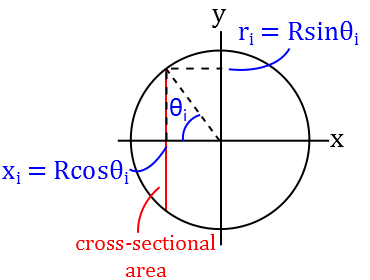
\includegraphics[width=0.4\linewidth]{Figures/Cross_sectional_area.png}
\caption{
Two-dimensional illustration of the three-dimensional problem of determining the density of particles in each $x$-value.
}
\label{fig:Cross_sectional_area}
\end{figure}
The cross-sectional area of the sphere in a specific area is found from a little trigonometry, by first considering that the radius of the circle that makes of the cross-sectional area in a point $x_i$ is given by $r_i = 20sin\theta_i$ ly.  
This yields that the area $A_i$ of the cross-sectional area, in ly, is given as
\begin{align}
	A_i = 400\pi sin^2 \theta_i =  400\pi (1 - cos^2 \theta)
\end{align}
in which the last equal sign stems from $1 = cos^2 \theta + sin^2 \theta$.
But $x_i = 20 cos \theta_i$ ly, giving
\begin{align}
	A_i = \pi (400 - x_i^2)
\end{align}
\begin{figure}[H]
\centering
	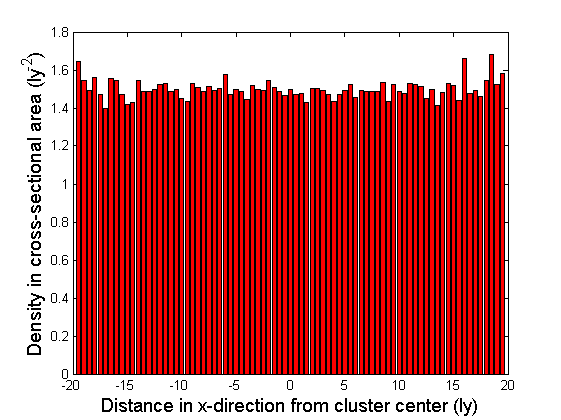
\includegraphics[width=0.7\linewidth]{Figures/random_uniform_position_test.png}
\caption{
Histogram of density of 100,000 particles with position generated by the code introduced in \fxnote{where??} as a function of the $x$-coordinate of the particles. The histogram is made with bins in the interval [$-19.5;19.5$] and a bin-size of $0.5$. The distance $x = \pm 20$ from the cluster center is not considered, since the cross-sectional area in that point is zero.
}
\label{fig:UniformlyGeneratedPos}
\end{figure}